\documentclass[a4paper,11pt]{article}
\usepackage{commonpackages}


\begin{document}
\title{Exercices avec Python - Turtle}
\date{}
\maketitle

\section{Introduction}
Le module turtle permet de faire des dessins. Nous allons l'utiliser pour comprendre et apprendre à utiliser différents concepts de programmation. Comme le résultat est visuel, c'est facile de savoir si ce que nous avons programmé fait ce qu'il faut.

\section{Exercice}
Dessiner une ligne traitillée en utilisant les fonctions penup() et pendown(). Ne pas oublier de les importer du module turtle.
\begin{solution}
\begin{code}[interactive_turtle]{python}
from turtle import *

for i in range(4):
    forward(20)
    penup()
    forward(20)
    pendown()
\end{code}
\end{solution}

\section{Exercice}
Dessiner un carré de 100 pixels en utilisant forward() et left() du module turtle.
\begin{solution}
\begin{code}[interactive_turtle]{python}
from turtle import *

forward(100)
left(90)
forward(100)
left(90)
forward(100)
left(90)
forward(100)
left(90)
\end{code}
\end{solution}

\section{Exercice}
Dessiner 2 carrés, de couleurs différentes et à des positions différentes, comme sur l'image ci-dessous.
\begin{multicols}{2}
\begin{enumerate}
\item Définir une fonction carre(nb_pixels) qui dessine un carré de 100 pixels de côté.
\item Utiliser la fonction goto(x,y) pour vous déplacer.
\item Utiliser 4 pixels pour l'épaisseur du trait.
\item Les couleurs du stylo sont noir (par défaut) et "blue".
\end{enumerate}
\begin{center}
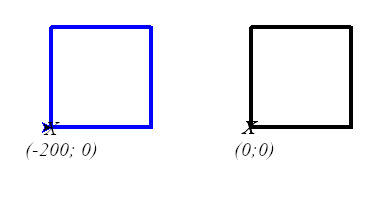
\includegraphics[width=0.8\textwidth]{images/TurtleCarres.png}\\
\end{center}
\end{multicols}

\begin{solution}
\begin{code}[interactive_turtle]{python}
from turtle import *

def carre(nb_pixels):
    for i in range(4):
        forward(nb_pixels)
        left(90)

pensize(4)
carre(100)
pencolor("blue")
penup()
goto(-200,0)
pendown()
carre(100)
\end{code}
\end{solution}

\section{Exercice}
\begin{multicols}{2}
Dessiner la forme ci-contre en utilisant une fonction tiangle(nb_pixels) qui dessine un triangle équilatéral de 100 pixels de côté.
\begin{center}
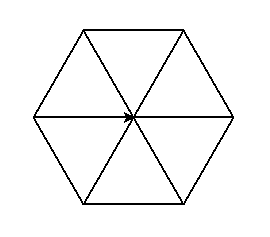
\includegraphics[width=0.8\textwidth]{images/Hexagone.png}\\
\end{center}
\end{multicols}

\begin{solution}
\begin{code}[interactive_turtle]{python}
from turtle import *

def triangle(nb_pixels):
    for i in range(3):
        forward(nb_pixels)
        left(120)

pensize(2)
for i in range(6):
    triangle(100)
    left(60)
\end{code}
\end{solution}

\end{document}
